\chapter{Results}

\begin{figure}
    \centering
    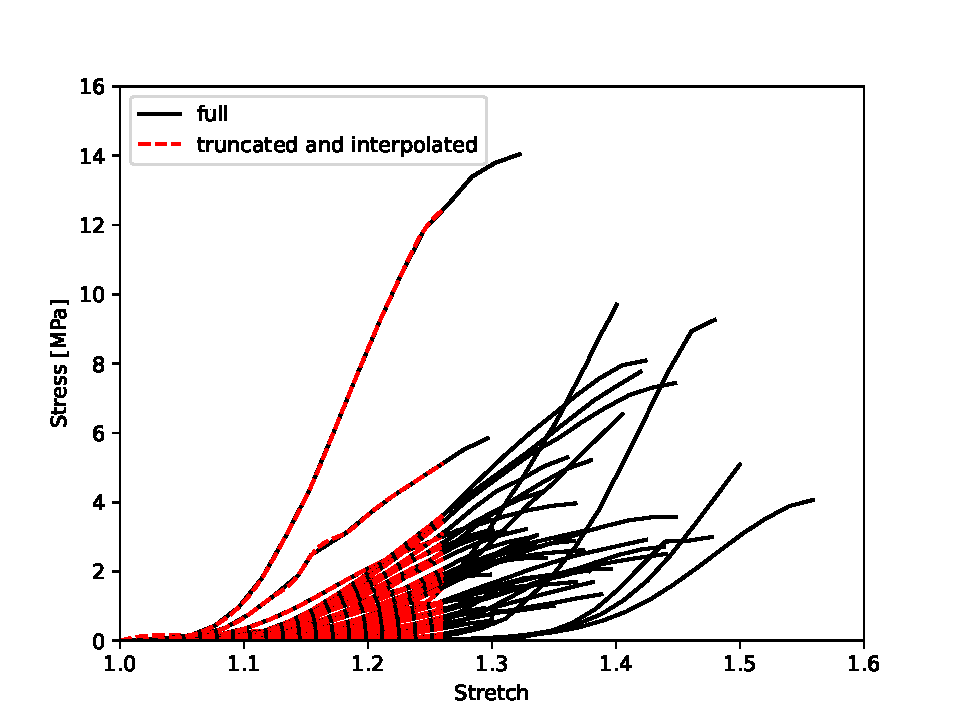
\includegraphics[width=\linewidth]{skinstression/images/truncated-and-interpolated-curves.pdf}
    \caption[Truncated and spline interpolated curves]{
        The strain-stress curves (black) were truncated and interpolated (dotted red)
        using non-uniform, interpolating splines on the stretch values of the curve with the lowest maximum stretch.
    }
    \label{fig:trunc_interp_curves}
\end{figure}

\section{Participants}

Earlier studies (refs) include 18 individuals (5 men, 4 women, and 6 unknown).
Abdomen data was excluded, because the strain-stress curves differ significantly from the thigh.
All thigh data is included, which is different from the original study, where only the 48 latest samples were used.
These considerations result in data including 15 individuals (5 men, 4 women, 3 unknown).
Ages range from 61 to 94.
Skin tissue is cut from the thigh and cut in multiple pieces of roughly the same shape.\marginpar{protocol?}
From every skin tissue piece, strain-stress curves are measured.
The number of measured strain-stress curves range from 1 to 13.
The source of data is summarized in table~\ref{tab:source_of_data}
\begin{table}
    \centering
    \caption[Source of data]{
        The selected individuals and their sex, age and number of strain-stress curves.
        - denotes unknown data.
    }
    \label{tab:source_of_data}
    \begin{tabular}{lllr}
        \toprule
        person & sex    & age & \# curves \\
        \midrule
        4      & -      & -   & 1         \\
        5      & male   & 61  & 1         \\
        6      & male   & 66  & 2         \\
        7      & male   & 79  & 1         \\
        8      & male   & 77  & 1         \\
        9      & male   & 75  & 1         \\
        10     & female & 94  & 1         \\
        11     & -      & -   & 1         \\
        12     & -      & -   & 1         \\
        13     & male   & 82  & 3         \\
        14     & female & 90  & 4         \\
        15     & female & 87  & 5         \\
        16     & male   & 95  & 12        \\
        17     & male   & 83  & 13        \\
        18     & female & 88  & 9         \\
        \bottomrule
    \end{tabular}
\end{table}